\documentclass[../main.tex]{subfiles}

\begin{document}

\chapter{Charged Particle Interaction Physics}
The interaction physics that describe the slowing down of energetic light ions through collisions with background charged particles in plasmas are described in terms of differential cross sections. The general differential cross section that describes a collision between an incident energetic light ion of species $x$ and a target charged particle of species $t$ resulting in new species $s$ is written as,
\begin{equation} \label{eqn:differential cross section}
    \sigma_{x,t \rightarrow s}(E^{\prime} \rightarrow E; \mucm),
\end{equation}
where the incident ion, $x$, had energy $E^{\prime}$ before its collision with the target species $t$. The resulting species $s$ is scattered through an angle whose CM cosine is $\mucm$ and has resulting energy $E$. Note the scattered species $s$ can be any species that results from the collision described by Eq. \eqref{eqn:differential cross section}. Collisions where the resulting species is identical to the incident species, $s = x$, are elastic scattering collisions; and collisions where the resulting species differs from the incident species, $s \neq x$, are called nuclear-reaction collisions. These nuclear-reaction collisions result in the destruction of the incident energetic light ions and are therefore considered absorption collisions for the incident ion. Furthermore, light ion collisions can either be described as light or heavy depending on whether the incident ion is lighter or heavier than the target particle respectively. Additionally, the differential cross section in Eq. \eqref{eqn:differential cross section} is referred to as the microscopic differential cross section and has units of $cm^{2}$, and is related to the macroscopic differential cross section as
\begin{equation}
    \Sigma_{x,t \rightarrow s}(E^{\prime} \rightarrow E; \mucm) = \mathcal{N} \sigma_{x,t \rightarrow s}(E^{\prime} \rightarrow E; \mucm),
\end{equation}
where $\mathcal{N}$ is the number density of the target species in $cm^{-3}$.

In general, as the energetic light ions slow down they experience four types of collisions with the background charged particles present in the plasma:
\begin{enumerate}
    \item elastic-Coulomb collisions with thermal electrons;
    \item elastic-Coulomb collisions with thermal ions;
    \item nuclear-elastic scattering (NES) collisions with thermal ions; or
    \item nuclear-reaction collisions with thermal ions.
\end{enumerate}
Because the ion-ion elastic scattering collisions consist of two parts (Coulomb and NES), a quantum mechanical interference differential cross section appears that describes the mutual interference between the two types of elastic scattering collisions \cite{Devaney-1971}. Therefore, the total elastic scattering differential cross section is written as
\begin{equation}
    \sigma_{x,t \rightarrow x} = \sigma_{x,t \rightarrow x}^C + \sigma_{x,t \rightarrow x}^N + \sigma_{x,t \rightarrow x}^I,
\end{equation}
where the superscripts $C$, $N$, and $I$ represent the Coulomb, NES, and interference components of the total ion-ion elastic scattering differential cross section. The differential cross sections that describe Coulomb collisions have an analytical form; while the differential cross sections that describe the NES, interference, and nuclear reactions collisions are tabulated in data sets. The remainder of this section presents the analytical form of the Coulomb differential cross section, and the forms of the tabulated differential cross sections describing the NES, interference, and nuclear-reaction collisions.

% ------------------------------------------------
% COULOMB DIFFERENTIAL CROSS SECTION
% ------------------------------------------------
\section{The Coulomb differential cross-section}
The Coulomb differential cross section describes the collisions that charged particles experience in a medium as a result of interaction with the charges of the background charged particles present in the plasma. These collisions are described by the Coulomb potential,
\begin{equation} \label{eqn:Coulomb_potential}
    V(r) = \dfrac{Z_1 \, Z_2 \, e^2}{r},
\end{equation}
where $Z_1 e$ and $Z_2 e$ are the charges of the incident and target charged particles, and $r$ is the distance between the two charges. The analytical form of the Coulomb differential cross section is found by applying the first-order Born approximation to the Schrodinger equation and using the Coulomb potential to describe the interaction potential \cite{Devaney-1971}. For unlike particles the Coulomb differential cross section is:
\begin{equation} \label{eqn:Coulomb}
    \sigma_{x,t \rightarrow x}^C(E^{\prime}\rightarrow E; \mucm) = \dfrac{\eta(E^{\prime})^2}{\kappa(E^{\prime}) (1 - \mucm)^2},
\end{equation}
where $\eta(E)$ is the dimensionless Coulomb parameter and $\kappa(E)$ is the incident particle's wave number given by
\begin{equation} \label{eqn:Coulomb_parameters}
    \eta(E) = Z_1 \, Z_2 \sqrt{\frac{\alpha^2 \, m_1 c^2}{2E}}, \quad 
    \kappa(E) = \dfrac{A}{A+1} \sqrt{\frac{2 \, m_1c^2 \, E}{(\hbar c)^2}}.
\end{equation}
In Eq.~\eqref{eqn:Coulomb_parameters}, $\alpha$ is the fine structure constant, $m_1 c^2$ is the mass of the incident ion, $A$ is the ratio of the target particle's mass to the incident particle's mass, and $\hbar c$ is Planck's reduced constant. For like particles, the Coulomb differential cross section depends on the spin of the particles, and its analytical form is given here \cite{Hale-1983}. Figure \ref{fig:sigma_c} shows a plot of Eq.~\eqref{eqn:Coulomb} for energetic deuterons colliding with tritons at an energy of 1 MeV. From Figure \ref{fig:sigma_c}, the analytical form of the Coulomb differential cross section, as described by Eq.~\eqref{eqn:Coulomb}, is highly peaked about zero angular-deflection and energy loss, and these collisions possess a small MFP. Furthermore from Eq.~\eqref{eqn:Coulomb}, the Coulomb differential cross section contains a singularity at $\mucm = 1$. This singularity results from the Coulomb potential, which allows for two particles that are infinitely far apart to interact with one another through their charges. This infinite interaction potential is not physical because, in realistic applications, charged particles are effectively screened by the surrounding charged particles and cannot interact with one another when they are infinitely far apart.

\begin{figure}[!htb]
    \centering
    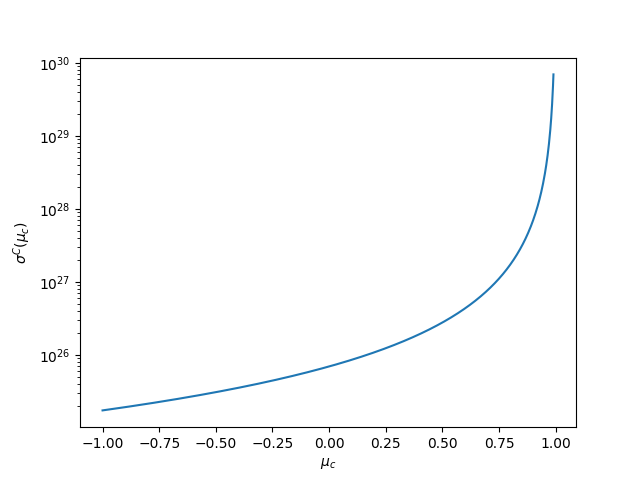
\includegraphics[scale=0.75]{boltzmann_model/Coulomb.png}
    \caption{Coulomb differential cross section for energetic deuterons colliding with tritons at 1.0 MeV cutoff at $\mucm = 0.99$}
    \label{fig:sigma_c}
\end{figure}


% ------------------------------------------------
% TABULATED DATA
% ------------------------------------------------
\section{The nuclear-elastic, interference, and nuclear-reaction differential cross sections}
The nuclear-elastic, interference, and nuclear-reaction differential cross sections do not have analytical forms, and are instead tabulated in data sets. In this work the LANL charged particle data sets are used, which are tabulated in the evaluated nuclear data format (ENDF) files \cite{Brown-2018}. The LANL charged particle data sets were selected because they contain interference differential cross sections that are evaluated over the full angular range and are not cut off when the interference differential cross section becomes negative \cite{Perkins-1981} \cite{Hale-1983}. In the ENDF files, the NES and nuclear-reaction differential cross sections are tabulated in terms of Legendre expansions as
\begin{equation} \label{eqn:nes_differential cross section}
    \sigma_{x,t \rightarrow x}^N(E^{\prime} \rightarrow E; \mucm) = \sum_{l=0}^L \dfrac{2l+1}{2} b_l(E^{\prime}) P_l(\mucm),
\end{equation}
and
\begin{equation}\label{eqn:nuclear-reaction_differential cross section}
    \sigma_{x,t \rightarrow s}(E^{\prime} \rightarrow E; \mucm) = \dfrac{1}{2} + \sum_{l=1}^N \dfrac{2l+1}{2} b_l(E^{\prime}) P_l(\mucm),
\end{equation}
where $P_l(\mucm)$ are the Legendre polynomials of order $l$, and $b_l(E)$ are the tabulated Legendre expansion coefficients. Similarly, the interference differential cross sections are expressed in the ENDF files in terms of a complex Legendre expansion as,
\begin{equation} \label{eqn:interference_differential cross section}
    \sigma_{x,t \rightarrow x}^I(E^{\prime} \rightarrow E; \mucm) = -\dfrac{2 \eta(E^{\prime})}{1 - \mucm} \text{Re} \left\lbrace \text{exp}\left[ i \eta(E^{\prime}) \text{ln}\left(\frac{1 - \mucm}{2} \right)\right] \sum_{l=0}^L \dfrac{2l+1}{2} a_l(E) P_l(\mucm) \right\rbrace,
\end{equation}
where $\eta(E)$ is the dimensionless Coulomb parameter given in Eq.~\eqref{eqn:Coulomb_parameters}, and $a_l(E)$ are the complex Legendre coefficients.

Figure \ref{fig:sig_n} shows a plot of the NES differential cross section for energetic deuterons colliding with tritons at various incident energies. From Figure \ref{fig:sig_n}, it can be concluded that at low incident ion energies NES is not an important collision effect, but as the incident energy of the particle increases NES collisions become important. Additionally, the NES differential cross sections allow for back-scattering collisions to occur when the incident energies of the ions are high enough. These back-scatter collisions produce energetic recoil ions that have been shown to be an important effect in the heating of the plasma \cite{Nakao-1988}. In general, it can be concluded that NES collisions are not highly peaked and that they have large MFPs when compared to the corresponding Coulomb differential cross sections.

In Figure \ref{fig:sig_i}, the interference differential cross section for energetic deuterons colliding with tritons is shown for various incident energies. Looking at Figure \ref{fig:sig_i}, as $\mucm \rightarrow 1$ the interference differential cross section oscillates between positive and negative values of increasing magnitude. Negative differential cross sections have no physical meaning, and therefore the interference differential cross section must be combined some other differential cross section such that the resulting differential cross section is always positive.

\begin{figure}[!htb]
    \centering
    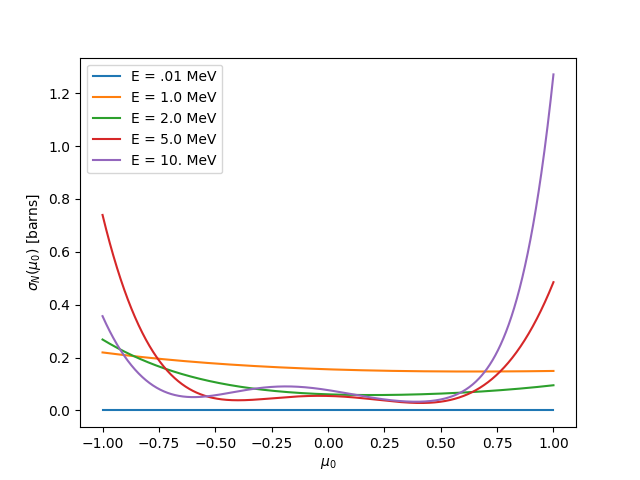
\includegraphics[scale=0.75]{proposed_work/sig_n_dt.png}
    \caption{Nuclear-elastic scattering differential cross section for deuterons colliding with tritons at 1.0 MeV}
    \label{fig:sig_n}
\end{figure}

\begin{figure}[!htb]
    \centering
    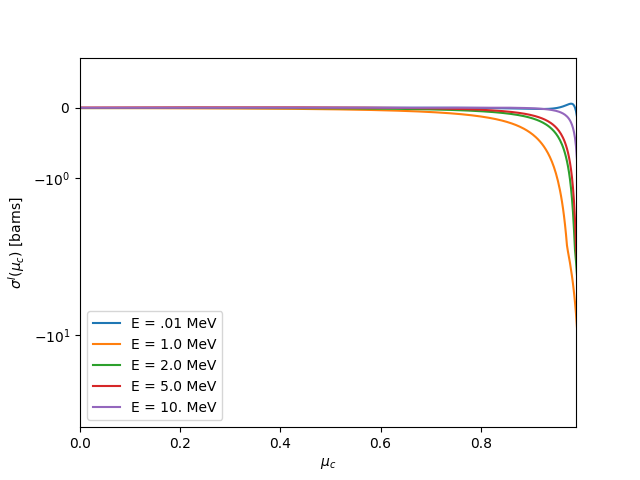
\includegraphics[scale=0.75]{proposed_work/sig_i_dt.png}
    \caption{Interference scattering differential cross section for deuterons colliding with tritons at 1.0 MeV}
    \label{fig:sig_i}
\end{figure}

Figures \ref{fig:sig_rt} and \ref{fig:sig_r} show plots of the total and differential nuclear-reaction cross sections for energetic deuterons colliding with tritons and producing energetic neutrons, that is, 
\begin{equation}
    \sigma_{D,T \rightarrow n}(E^{\prime} \rightarrow E; \mucm).
\end{equation}
This DT nuclear-reaction collision also results in the production of an energetic $\alpha$-particle, but this cross section is not directly tabulated in the ENDF files and two-body kinematics are needed to calculate the corresponding differential cross section. From Figure \ref{fig:sig_rt}, the DT fusion reaction clearly has a threshold for reaction of about 0.02 MeV and a peak for incident deuterons of 0.1 MeV. Furthermore, looking at Figure \ref{fig:sig_r}, the neutrons that are produced are almost nearly isotropic in angle. While this DT nuclear-reaction cross section only represents one possible type of charged particle collision, the general comment that can be made is that charged-particle nuclear-reaction differential cross sections are not highly peaked and that these types of collisions have large MFPs when compared to the Coulomb differential cross sections.

\begin{figure}[!htb]
    \centering
    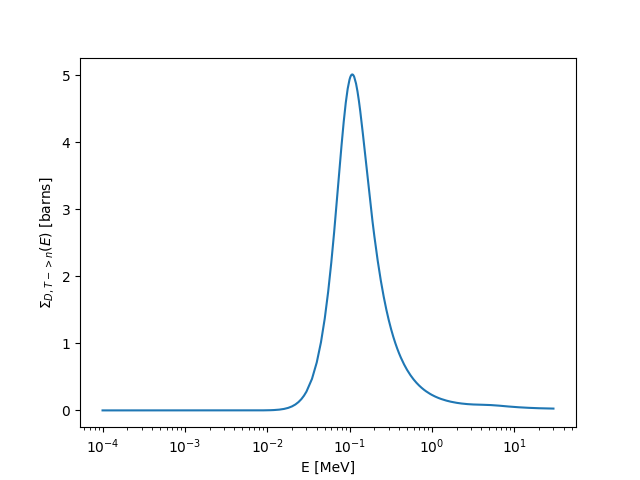
\includegraphics[scale=0.75]{boltzmann_model/DT_TotalReactionXS.png}
    \caption{Total nuclear-reaction cross section for $D+T \rightarrow n$}
    \label{fig:sig_rt}
\end{figure}

\begin{figure}[!htb]
    \centering
    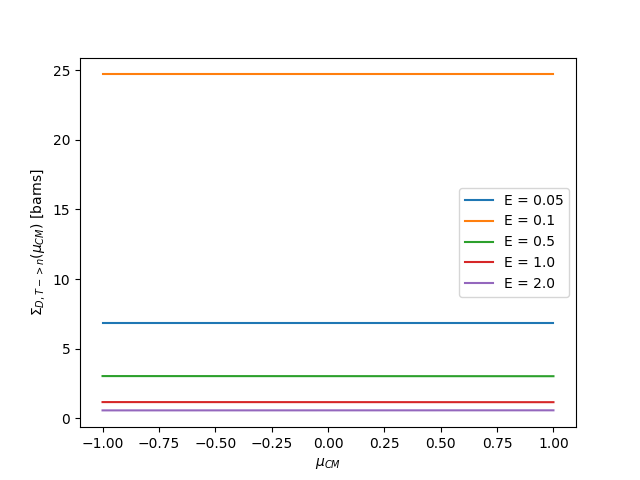
\includegraphics[scale=0.75]{boltzmann_model/DT_ReactionXS.png}
    \caption{Nuclear-reaction differential cross section for $D+T \rightarrow n$}
    \label{fig:sig_r}
\end{figure}

% \section{Coulomb Differential Cross Sections}
% \subsection{Unscreened Coulomb differential cross sections}
% The scattering amplitude for a Coulomb potential in Coulomb units is:
% \begin{equation}
%     f(\theta) = \dfrac{\gamma}{2 \, k \, \sin^2 \theta/2} \exp \left[ 2 \, i \, \gamma \, \log \sin \theta/2 \right] \dfrac{\Gamma(1 + i/k)}{\Gamma(1 - i/k)}
% \end{equation}
% where $\gamma = Z_1 \, Z_2 \, e^2 / \hbar \, v$, $v$ being the incident velocity, and $\hbar \, k = \mu \, v$.

% \subsubsection{Distinguishable particles}
% For distinguishable particles the differential cross section is given by:
% \begin{equation}
%     \sigma_{C,d} = | f(\theta) |^2 = f(\theta) \, f^{\star}(\theta)
% \end{equation}
% To begin we rewrite the exponential term using Euler's formula as:
% \begin{equation}
%     f(\theta) = \dfrac{\gamma}{2 \, k \, \sin^2 \theta/2} \left[ \cos x_1 + i \, \sin x_1 \right] \dfrac{\Gamma(1 + i/k)}{\Gamma(1 - i/k)}, \quad x_1 =  2 \, \gamma \, \log \sin \theta/2
% \end{equation}
% The complex conjugate of the scattering amplitude is:
% \begin{equation}
%     f^{\star}(\theta) = \dfrac{\gamma}{2 \, k \, \sin^2 \theta/2} \left[ \cos x_1 - i \, \sin x_1 \right] \dfrac{\Gamma(1 - i/k)}{\Gamma(1 + i/k)}, \quad x_1 =  2 \, \gamma \, \log \sin \theta/2
% \end{equation}
% Substituting in the scattering amplitude and the complex conjugate of the scattering amplitude gives:
% \begin{multline}
%     \sigma_{C,d} = \left\lbrace \dfrac{\gamma}{2 \, k \, \sin^2 \theta/2} \left[ \cos x_1 + i \, \sin x_1 \right] \dfrac{\Gamma(1 + i/k)}{\Gamma(1 - i/k)} \right\rbrace \\
%     \times \left\lbrace \dfrac{\gamma}{2 \, k \, \sin^2 \theta/2} \left[ \cos x_1 - i \, \sin x_1 \right] \dfrac{\Gamma(1 - i/k)}{\Gamma(1 + i/k)} \right\rbrace
% \end{multline}
% Simplifying gives:
% \begin{equation}
%    \sigma_{C,d} = \dfrac{\gamma^2}{4 \, k^2 \, \sin^4 \theta/2}
% \end{equation}
% Finally, substituting in the expression for $\gamma$ and $k$ gives:
% \begin{equation} \label{eqn:dist_unscreened_coulomb}
%     \boxed{ \sigma_{C,d} = \left(\dfrac{Z_1 \, Z_2 \, e^2}{2 \, \mu \, v_1^2}\right)^2 \dfrac{1}{\sin^4 \theta/2} }
% \end{equation}

% To get Eq. \eqref{eqn:dist_unscreened_coulomb} into a more readily usable form (form in the ENDF manual), we begin by rewriting $e^2 = \alpha \, \hbar c$ and using the half angle trigonometry identity $2 \sin^2 \theta / 2 = 1 - \cos \theta$ giving:
% \begin{equation}
%     \sigma_{C,d} = \left(\dfrac{Z_1 \, Z_2 \, \alpha \, \hbar c}{\mu \, v_1^2}\right)^2 \dfrac{1}{(1 - \mu_0)^2}, \quad \text{where} \,\, \mu_0 = \cos \theta
% \end{equation}
% Next expanding out the reduced mass as $\mu = \dfrac{m_1 m_2}{m_1 + m_2}$ gives:
% \begin{equation}
%     \sigma_{C,d} = \left(\dfrac{Z_1 \, Z_2 \, \alpha \, \hbar c}{ \left(\frac{A}{1 + A} \right) \, m_1 \, v_1^2}\right)^2 \dfrac{1}{(1 - \mu_0)^2}, \quad \text{where} \,\, A = \dfrac{m_2}{m_1}.
% \end{equation}
% Using $m_1 \, v_1^2 = 2 \, E$ gives:
% \begin{equation}
%     \sigma_{C,d} = \left(\dfrac{Z_1^2 \, Z_2^2 \, \left(\alpha \, \hbar c\right)^2}{ 4 \, E^2 \, \left(\frac{A}{1 + A} \right)^2}\right) \dfrac{1}{(1 - \mu_0)^2}.
% \end{equation}

% \subsubsection{Identical particles}
% For identical particles the differential cross section is given by:
% \begin{equation} \label{eqn:formula-identical-particles}
%      \sigma_{C,i} = | f(\theta) |^2 + | f(\pi - \theta) |^2 + \dfrac{(-1)^{2s}}{2s+1} \left[ f(\theta) f^{\star}(\pi-\theta) + f^{\star}(\theta) f(\pi-\theta) \right]
% \end{equation}
% In the above equation we already know $f(\theta)$ and $f^{\star}(\theta)$, to get $f(\pi-\theta)$ we simply substitute in $\theta = \pi - \theta$ to get
% \begin{equation}
%     f(\pi - \theta) = \dfrac{\gamma}{2 \, k \, \sin^2 \left(\frac{\pi - \theta}{2} \right)} \exp \left[ 2 \, i \, \gamma \, \log \sin \left(\frac{\pi - \theta}{2} \right) \right] \dfrac{\Gamma(1 + i/k)}{\Gamma(1 - i/k)}
% \end{equation}
% Note that:
% \begin{equation*}
%     \sin \left(\frac{\pi - \theta}{2} \right) = \sin \left(\dfrac{\pi}{2} - \dfrac{\theta}{2}\right) = \cos \theta/2
% \end{equation*}
% and therefore the shifted scattering amplitude is simply
% \begin{equation}
%     f(\pi - \theta) = \dfrac{\gamma}{2 \, k \, \cos^2 \theta/2} \exp \left[ 2 \, i \, \gamma \, \log \cos \theta/2 \right] \dfrac{\Gamma(1 + i/k)}{\Gamma(1 - i/k)},
% \end{equation}
% Using Euler's formula the shifted scattering amplitude and complex conjugate of the scattering amplitude can be rewritten as
% \begin{equation}
%     f(\pi - \theta) = \dfrac{\gamma}{2 \, k \, \cos^2 \theta/2} \left[ \cos x_2 + i \, \sin x_2 \right] \dfrac{\Gamma(1 + i/k)}{\Gamma(1 - i/k)}, \quad x_2 =  2 \, \gamma \, \log \cos \theta/2
% \end{equation}
% and
% \begin{equation}
%     f^{\star}(\pi - \theta) = \dfrac{\gamma}{2 \, k \, \cos^2 \theta/2} \left[ \cos x_2 - i \, \sin x_2 \right] \dfrac{\Gamma(1 - i/k)}{\Gamma(1 + i/k)}, \quad x_2 =  2 \, \gamma \, \log \cos \theta/2
% \end{equation}

% From the previous section the first term in Eq. \eqref{eqn:formula-identical-particles} is simply
% \begin{equation}
%     | f(\theta) |^2 = \dfrac{\gamma^2}{4 \, k^2 \, \sin^4 \theta/2}
% \end{equation}
% and similarly the second term in Eq. \eqref{eqn:formula-identical-particles} is
% \begin{equation}
%     | f(\pi - \theta) |^2 = \dfrac{\gamma^2}{4 \, k^2 \, \cos^4 \theta/2}
% \end{equation}
% Substituting in the scattering amplitudes into the third term in Eq. \eqref{eqn:formula-identical-particles} gives:
% \begin{multline}
%     \left[ f(\theta) f^{\star}(\pi-\theta) + f^{\star}(\theta) f(\pi-\theta) \right] = \left\lbrace \dfrac{\gamma}{2 \, k \, \sin^2 \theta/2} \left[ \cos x_1 + i \, \sin x_1 \right] \dfrac{\Gamma(1 + i/k)}{\Gamma(1 - i/k)} \right\rbrace \\
%     \times \left\lbrace \dfrac{\gamma}{2 \, k \, \cos^2 \theta/2} \left[ \cos x_2 - i \, \sin x_2 \right] \dfrac{\Gamma(1 - i/k)}{\Gamma(1 + i/k)} \right\rbrace \\
%     + \left\lbrace \dfrac{\gamma}{2 \, k \, \sin^2 \theta/2} \left[ \cos x_1 - i \, \sin x_1 \right] \dfrac{\Gamma(1 - i/k)}{\Gamma(1 + i/k)} \right\rbrace \\
%     \times \left\lbrace \dfrac{\gamma}{2 \, k \, \cos^2 \theta/2} \left[ \cos x_2 + i \, \sin x_2 \right] \dfrac{\Gamma(1 + i/k)}{\Gamma(1 - i/k)} \right\rbrace
% \end{multline}
% Simplifying and collecting like terms gives:
% \begin{multline}
%     \left[ f(\theta) f^{\star}(\pi-\theta) + f^{\star}(\theta) f(\pi-\theta) \right] = \\
%     \dfrac{\gamma^2}{4 \, k^2 \, \sin^2 \left(\theta/2 \right) \, \cos^2 \left(\theta/2\right)} \left[ \left( \cos x_1 + i \, \sin x_1 \right) \left( \cos x_2 - i \, \sin x_2 \right) \right. \\ \left. + \left( \cos x_1 - i \, \sin x_1 \right) \left( \cos x_2 + i \, \sin x_2 \right) \right]
% \end{multline}
% Expanding the expression and simplifying gives
% \begin{equation}
%     \left[ f(\theta) f^{\star}(\pi-\theta) + f^{\star}(\theta) f(\pi-\theta) \right] = \dfrac{2 \, \gamma^2}{4 \, k^2 \, \sin^2 \left(\theta/2 \right) \, \cos^2 \left(\theta/2\right)} \left[ \cos x_1 \, \cos x_2 + \sin x_1 \, \sin x_2  \right]
% \end{equation}
% Next using the trig identity $\cos (\alpha - \beta) = \cos \alpha \, \cos \beta + \sin \alpha \, \sin \beta$ the above expression simplifies to:
% \begin{equation}
%     \left[ f(\theta) f^{\star}(\pi-\theta) + f^{\star}(\theta) f(\pi-\theta) \right] = \dfrac{2 \, \gamma^2}{4 \, k^2 \, \sin^2 \left(\theta/2 \right) \, \cos^2 \left(\theta/2\right)} \cos \left( x_1 - x_2  \right)
% \end{equation}
% Substituting in our expression for $x_1$ and $x_2$ gives:
% \begin{equation}
%     \cos \left( x_1 - x_2  \right) = \cos \left[ 2 \, \gamma \, \left( \log \sin \theta/2 -  \log \cos \theta/2 \right)  \right]
% \end{equation}
% which readily simplifies to 
% \begin{equation}
%     \cos \left( x_1 - x_2  \right) = \cos \left( \gamma \, \log \, \tan^2 \theta/2 \right)
% \end{equation}

% Putting everything together we arrive at the final differential cross section for identical particles
% \begin{equation}
%     \sigma_{C,i} = \dfrac{\gamma^2}{4 \, k^2} \left[ \dfrac{1}{\sin^4 \theta/2} + \dfrac{1}{\cos^4 \theta/2} + \dfrac{(-1)^{2s}}{2s+1} \dfrac{2}{\sin^2 \left(\theta/2 \right) \, \cos^2 \left(\theta/2\right)} \cos \left( \gamma \, \log \, \tan^2 \theta/2 \right) \right]
% \end{equation}
% Next using the trig half-angle identities and $\mu_0 = \cos \theta$ gives:
% \begin{equation} \label{eqn:coulomb-unscreened-identical}
%     \boxed{ \sigma_{C,i} = \dfrac{\gamma^2}{k^2} \left[ \dfrac{1}{(1 - \mu_0)^2} + \dfrac{1}{(1 + \mu_0)^2} + \dfrac{(-1)^{2s}}{2s+1} \dfrac{2}{(1 - \mu_0)(1 + \mu_0)} \cos \left( \gamma \, \log \, \dfrac{1 - \mu_0}{1 + \mu_0} \right) \right] }
% \end{equation}
% Note, Eq. \eqref{eqn:coulomb-unscreened-identical} can be written in the form that appears in the ENDF manual by factoring out $2 / (1 - \mu_0^2)$ giving:
% \begin{equation}
%     \sigma_{C,i} = \dfrac{2 \, \gamma^2}{k^2 (1 - \mu_0^2)} \left[ \dfrac{1+\mu_0^2}{1-\mu_0^2} + \dfrac{(-1)^{2s}}{2s+1} \cos \left( \gamma \, \log \, \dfrac{1 - \mu_0}{1 + \mu_0} \right) \right]
% \end{equation}

% \subsection{Screened coulomb differential cross sections}
% The scattering amplitude is given through Born approximation as
% \begin{equation}
%     f_W = - \dfrac{2 \, m}{\hbar^2} \int\limits_0^{\infty} U(r) \, \dfrac{\sin qr}{q} \, r \, dr
% \end{equation}
% where $q = 2 \, k \, \sin \theta / 2$. The Wentzel scattering potential is:
% \begin{equation}
%     U(r) = \dfrac{Z_1 \, Z_2 \, e^2}{r} \, \exp \left(-r/R\right)
% \end{equation}
% Substituting this potential into the scattering amplitude equation gives:
% \begin{equation}
%     f_W = - \dfrac{2 \, Z_1 \, Z_2 \, e^2 \, m}{q \, \hbar^2} \int\limits_0^{\infty} \, \sin qr \, \exp \left(-r/R\right) \, dr
% \end{equation}
% Expanding the sin function in the integral using Euler's formula gives:
% \begin{equation}
%    \dfrac{1}{2 \, i} \int\limits_0^{\infty} \, \Big\lbrace \text{e}^{-(\frac{1}{R} - i\,q)r} - \text{e}^{-(\frac{1}{R} + i\,q)r} \Big\rbrace \, dr
% \end{equation}
% Preforming the integration gives
% \begin{equation}
%     \dfrac{1}{2 \, i} \left[ \dfrac{i \, R}{i + q \, R} - \dfrac{i \, R}{i - q \, R} \right] = \dfrac{1}{2 \, i} \left[ \dfrac{2 \, i \, q \, R^2}{1 + q^2 \, R^2}\right] = \dfrac{q \, R^2}{1 + q^2 \, R^2} = \dfrac{q}{\left(\frac{1}{R}\right)^2 + q^2}
% \end{equation}
% Finally, substituting the above expression back into the scattering amplitude expression  gives
% \begin{equation}
%     f_W = - \dfrac{2 \, Z_1 \, Z_2 \, e^2 \, m}{\hbar^2} \dfrac{1}{\left(1 / R\right)^2 + q^2} = - \dfrac{2 \, Z_1 \, Z_2 \, e^2 \, m}{\hbar^2} \dfrac{1}{\left(1 / R\right)^2 + 4 \, k^2 \, \sin^2 \theta / 2}
% \end{equation}
% Factoring out $\frac{1}{4 \, k^2}$ and inserting our expression for $\gamma$ and $k$ gives the final form of the screened Rutherford or ``Wentzel'' scattering amplitude as
% \begin{equation}
%     \boxed{f_W = - \dfrac{Z_1 \, Z_2 \, e^2 \, m}{2 \, k^2 \, \hbar^2} \dfrac{1}{(2kR)^{-2} + \sin^2 \theta/2} = - \dfrac{\gamma}{2 \, k} \left[\dfrac{1}{(2kR)^{-2} + \sin^2 \theta/2}\right]}
% \end{equation}

% \subsubsection{Distinguishable particles}
% For distinguishable particles the differential cross section is given by:
% \begin{equation}
%     \sigma_{W,d} = | f_W(\theta) |^2 = f_W(\theta) \, f_W^{\star}(\theta)
% \end{equation}
% Substituting in the Wentzel scattering amplitude gives the screened Coulomb or ``Wntzel'' differential cross as
% \begin{equation}
%     \boxed{\sigma_{W,d} = \dfrac{\gamma^2}{4 \, k^2} \dfrac{1}{\left[(2kR)^{-2} + \sin^2 \theta/2\right]^2} =  \dfrac{\gamma^2}{k^2} \dfrac{1}{\left[A_s + 1 - \mu_0\right]^2}}
% \end{equation}
% where $A_s = \left(\frac{1}{k \, R}\right)^2$ and $\mu_0 = \cos \theta$.

% \subsubsection{Identical particles}
% For identical particles the differential cross section is given by:
% \begin{equation}
%      \sigma_{W,i} = | f_W(\theta) |^2 + | f_W(\pi - \theta) |^2 + \dfrac{(-1)^{2s}}{2s+1} \left[ f_W(\theta) f_W^{\star}(\pi-\theta) + f_W^{\star}(\theta) f_W(\pi-\theta) \right]
% \end{equation}
% The shifted Wentzel screening amplitude is obtained by substituting $\theta = \pi - \theta$ into the Wentzel screening amplitude to get:
% \begin{equation}
%     f_W(\pi - \theta) = - \dfrac{\gamma}{2 \, k} \left[\dfrac{1}{(2kR)^{-2} + \cos^2 \theta/2}\right]
% \end{equation}
% Substituting in the Wentzel screening amplitudes into the equation for the differential cross section gives:
% \begin{multline}
%      \sigma_{W,i} = \dfrac{\gamma^2}{4 \, k^2} \left\lbrace \dfrac{1}{\left[(2kR)^{-2} + \sin^2 \theta/2\right]^2} + \dfrac{1}{\left[(2kR)^{-2} + \cos^2 \theta/2\right]^2}  \right. \\ \left.
%      + \dfrac{(-1)^{2s}}{2s+1} \dfrac{2}{\left[(2kR)^{-2} + \sin^2 \theta/2\right]\left[(2kR)^{-2} + \cos^2 \theta/2\right] }\right\rbrace
% \end{multline}
% Finally, substituting in $2 \sin^2 \theta/2 = 1 - \cos \theta$ and $2 \cos^2 \theta/2 = 1 + \cos \theta$ gives the final form of the Wentzel differential cross section for identical particles as:
% \begin{equation}
%      \boxed{\sigma_{W,i} = \dfrac{\gamma^2}{k^2} \left[ \dfrac{1}{\left(A_s + 1 - \mu_0\right)^2} + \dfrac{1}{\left(A_s + 1 + \mu_0\right)^2} + \dfrac{(-1)^{2s}}{2s+1} \dfrac{2}{\left(A_s + 1 - \mu_0\right)\left(A_s + 1 + \mu_0\right) }\right]}
% \end{equation}
% where $A_s = \left(\frac{1}{k \, R}\right)^2$ and $\mu_0 = \cos \theta$.
\end{document}
